%---------------------------------------------------------------------------
% Monitoring Hub component.
%
%---------------------------------------------------------------------------


\section{Monitoring Hub}
\label{sec:ch5_monitoring_hub}


Monitoring Hub is the core component of system. If using layered model to analyze application, Monitoring Hub should be
treated as logic layer - it is placed between presentation layer (GUI) and data access layer (transport proxies). It
provides services to GUI, like resources management (registering new resources, discovery dependent resources),
measurements management (creation, pausing, resuming and termination). It is also responsible for creating scheduled
jobs that pools for capability values and pushes new values to registered listeners. 

When user wants to start monitoring new resource, he or she must choose which Monitoring Hub will be used to monitor
given resource. It creates direct association between chosen Hub and resource bing monitored with all it's
child resources discovered during registration. This association ensures, that all calls to get current capability
values, or to manage measurements related to given resource will be processed by Monitoring Hub configured during
it's registration or discovery.

To allow loose coupling between components, Monitoring Hub doesn't know details about other components. To be able to
provide it's services it uses transport proxies and knowledge components, but it interacts with them only using
commonly known interfaces. Additionally it isn't aware about GUI components at all - it just provides services by
implementing given interface, and to be able to notify about variety of events, it uses also common listener
interfaces.

\subsection{Decomposition of Monitoring Hub}

\begin{figure}[h]
  \centering
  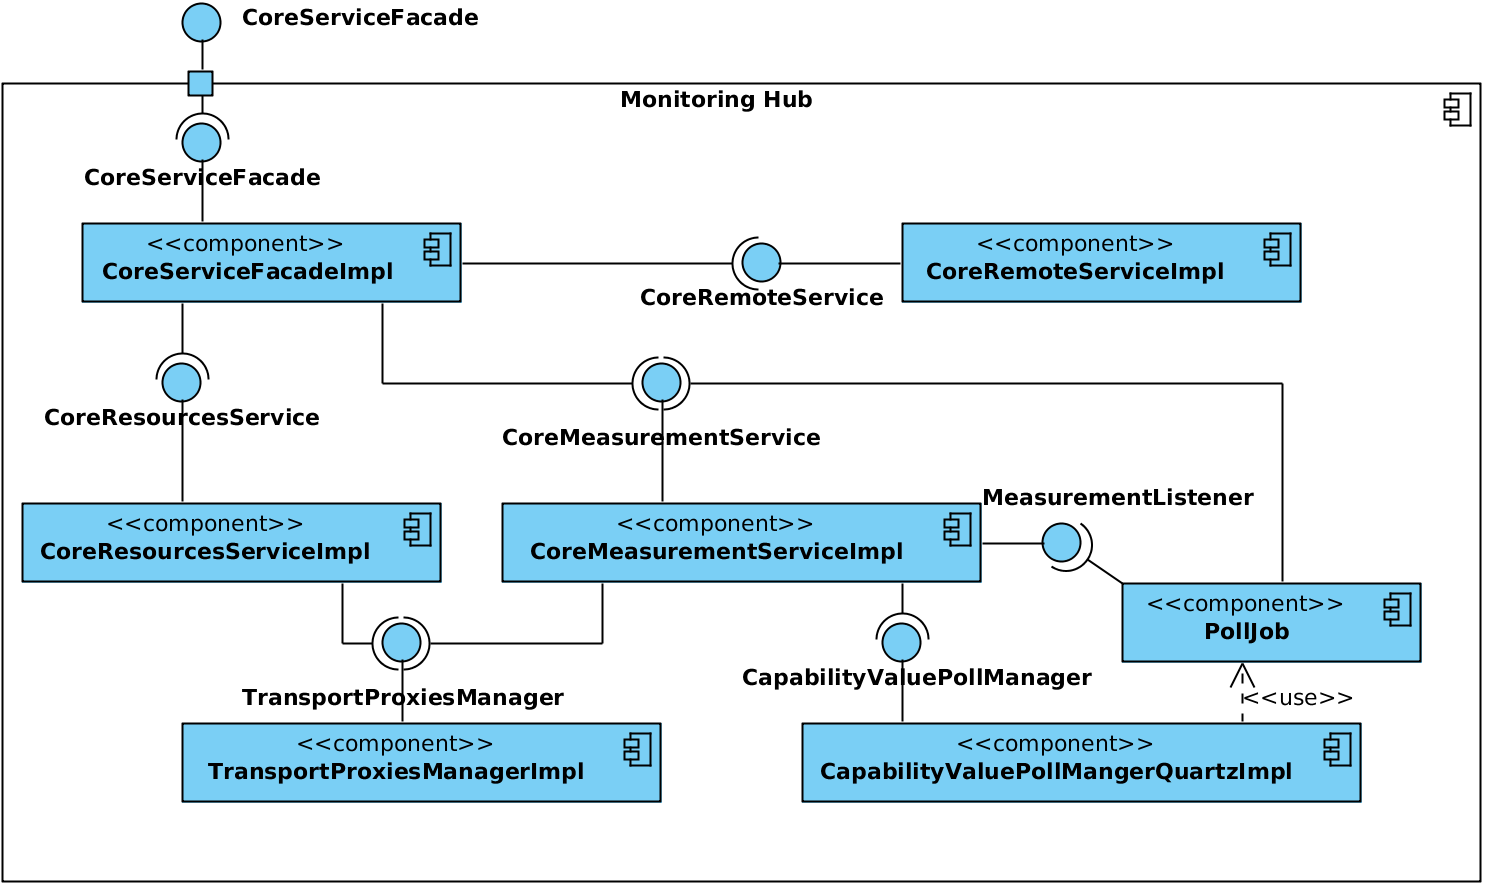
\includegraphics[width=0.9\textwidth]{decomposition_mon_hub}
  \caption{Communication diagram - adding of new resource}
  \label{fig:decomposition_mon_hub}
\end{figure}

Further decomposition of application, details of Monitoring Hub can be found in Figure~\ref{fig:decomposition_mon_hub}.
This component uses following subcomponents (with interfaces):

\begin{itemize}

 \item {\bf CoreServiceFacadeImpl}~~~~~~~~~~~~~~~~~~~~~~~~~~~~~~~~~~~~~~~~~~~~~~~~~~~~~~~~\linebreak
Facade that allows access to all Monitoring Hub functionalities from single interface (CoreServiceFacade, shared with
GUI and Monitoring Hub Application high level components). This wrapper is needed to ease remote access - exposing
and using one interface with any remoting middleware is easier than multiple interfaces, which in most cases would
require multiple socket connections. We should tend to use as small amount connections as possible, because more
connections are being used, than system becomes more and more prone to network configuration issues (e.g. firewalls).
Additionally, suing single facade improves code style, as with facade, only one interface has to be visible for all
components that are using services of given component.

 \item {\bf CoreRemoteServiceImpl}~~~~~~~~~~~~~~~~~~~~~~~~~~~~~~~~~~~~~~~~~~~~~~~~~~~~~~~~\linebreak
Service responsible for processing requests related to remote management of Monitoring Hub. It has two main
responsibilities, namely it allows to register remote listening interfaces and it dispatches local events (new resource,
new capability value etc.) to remote listeners in aggregated manner. Distributed dispatch of events requires a bit
different approach than local one (local one, means dispatch inside of single JVM process). First of all, in most cases
remote interface that will receive notifications in most cases uses different signature, to allow handling exceptions
related to networking. Additionally, to reduce amount of remote calls and thus improve efficiency,
CoreRemoteServiceImpl aggregates events into batches and notifies remote listeners using such a package of events. Such
an approach doesn't pollute measuring results, because each measurement value is associated with creation timestamp,
initialized by component that grabs given value, at the moment, when read of capability value is performed.
Additionally, as events related to resources addition/removal doesn't require 

 \item {\bf CoreResourcesServiceImpl}~~~~~~~~~~~~~~~~~~~~~~~~~~~~~~~~~~~~~~~~~~~~~~~~~~~~~~~~\linebreak
Service responsible for resources management - registering new resources, discovery of sub resources, and getting all
registered and discovered. It's also used to get more details about resource, like capabilities that given resource may
have.


 \item {\bf CoreMeasurementServiceImpl}~~~~~~~~~~~~~~~~~~~~~~~~~~~~~~~~~~~~~~~~~~~~~~~~~~~~~~~~\linebreak
Measurement services - can be used to create/pause/stop/terminate measurement, gather current values of capabilities.
It's used by PollJob for that purpose. Additionally it provides MeasurementListener interface so it can be notified
about new capability values polled by PollJob. 

 \item {\bf TransportProxiesManagerImpl}~~~~~~~~~~~~~~~~~~~~~~~~~~~~~~~~~~~~~~~~~~~~~~~~~~~~~~~~\linebreak
Manages registered transport proxies. It's used by other components to get all transport proxies, to get transport
proxy that can be used to manage given resource.

 \item {\bf CapabilityValuePollManagerImpl}~~~~~~~~~~~~~~~~~~~~~~~~~~~~~~~~~~~~~~~~~~~~~~~~~~~~~~~~\linebreak
Is responsible for scheduling polling jobs needed to run measurement.

 \item {\bf PollJob}~~~~~~~~~~~~~~~~~~~~~~~~~~~~~~~~~~~~~~~~~~~~~~~~~~~~~~~~\linebreak
Job triggered with configured interval, that simply polls for current capability value and push it to listeners.


\end{itemize}

\pagebreak

\subsection{Most important data flows}

This section contains description of most important data flows inside Monitoring Hub component. Following actions are
covered: adding new resources, adding new measurements  and new capability value notification.

Figure~\ref{fig:comm_mh_add_res} contains communication diagram of adding new resources. In this scenario, external GUI
components is initiator of action - first step is it's call registerResource to CoreServiceFacadeImpl. Facade simply
delegates this call to it's component - CoreResourcesServiceImpl, where adding of resource will be actually performed.
In next step, CoreResourcesServiceImpl tries to find proxy capable to communicate with given resource. To achieve that
it calls TransportProxiesManagerImpl. After successfully obtaining transport proxy, which is external component for
monitoring hub, resources service performs call on it to register given resource. If this registration succeeds,
resources service uses another external component, namely Knowledge, to get all types of possible children resources
that added resource may have. Using list of children types, resources service requests TransportProxy to discover all
children of resource being added. After successful discovery, notification containing resources id dispatched to all
listeners either directly, when given Monitoring Hub is embedded into GUI, or using CoreRemoteServiceImpl to dispatch to
all remote GUI components registered.

\begin{figure}[h]
  \centering
  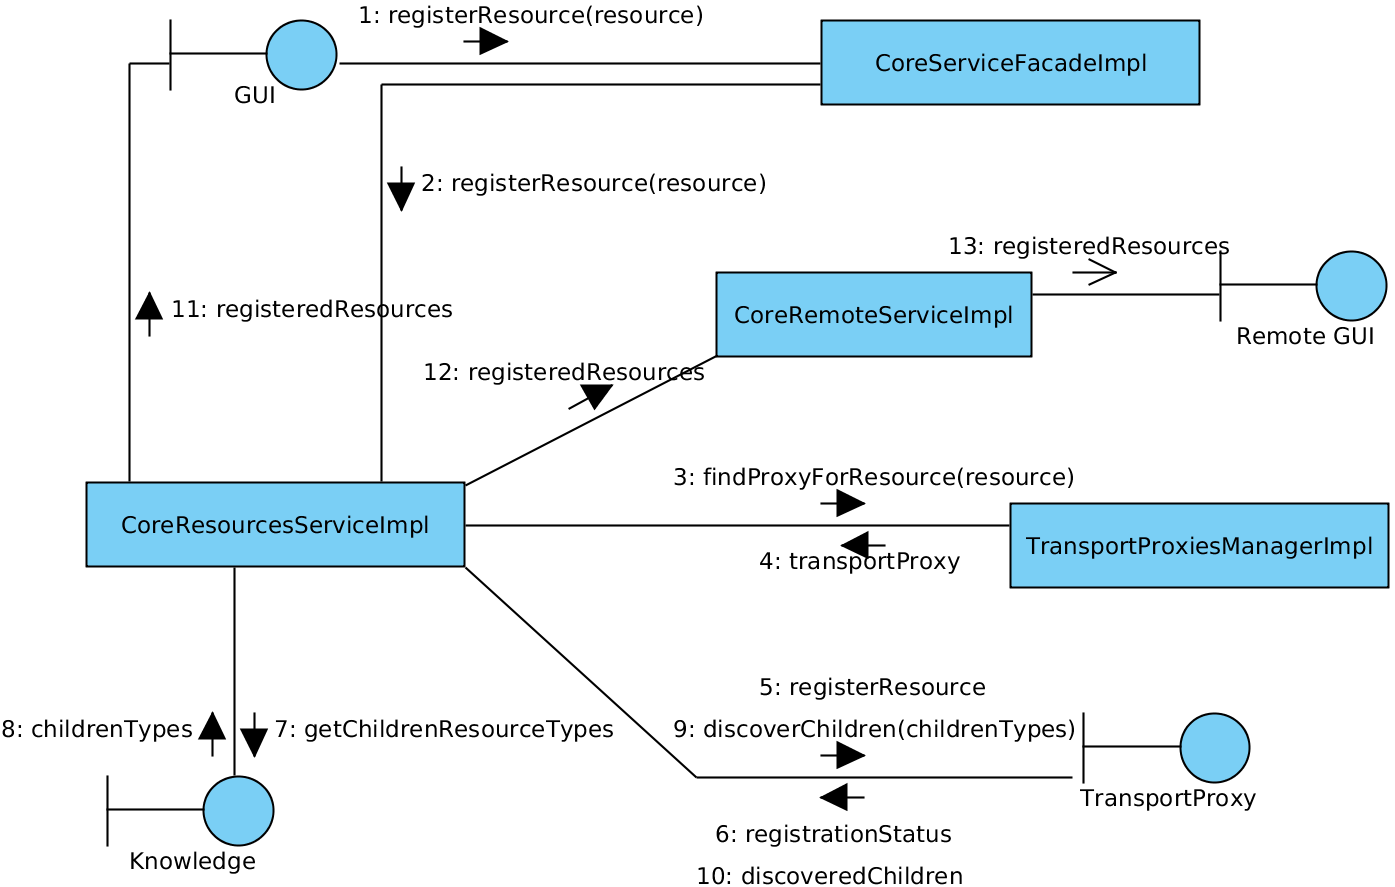
\includegraphics[width=0.9\textwidth]{comm_mh_add_res}
  \caption{Monitoring Hub Communication diagram - adding new resource}
  \label{fig:comm_mh_add_res}
\end{figure}



Communication diagram of adding new measurement action can be found in Figure~\ref{fig:comm_mh_add_measurement}. In
this scenario, again GUI is initiator of action. First request is made to CoreServiceFacadeImpl - GUI calls it's method
getResourceCapabilities, to allow user choose which capability he would like to create. Facade delegates query to
CoreResourcesServiceImpl, which passes it to external Knowledge component. Resulting list of capability URI's is being
passed all way back, to the GUI component. Next, user selects which capability should be measured, which makes GUI to
request CoreServiceFacadeImpl to create measurement using given definition (see Table~\ref{tab:TO_MeasurementDef} to
get request content). Request is delegated to CoreMeasurementServiceImpl which is responsible for actual creation of
measurement. Measurement service request CapabilityValuePollManagerImpl for creation of new PollJob. After
creating polling job, measurement service generates measurement id, stores it internally with measurement
definition, and returns it to requester. This Id is then passed back to GUI, so this component can use it to reference
incoming CapabilityValues and to be able to update or remove measurement.

\begin{figure}[h]
  \centering
  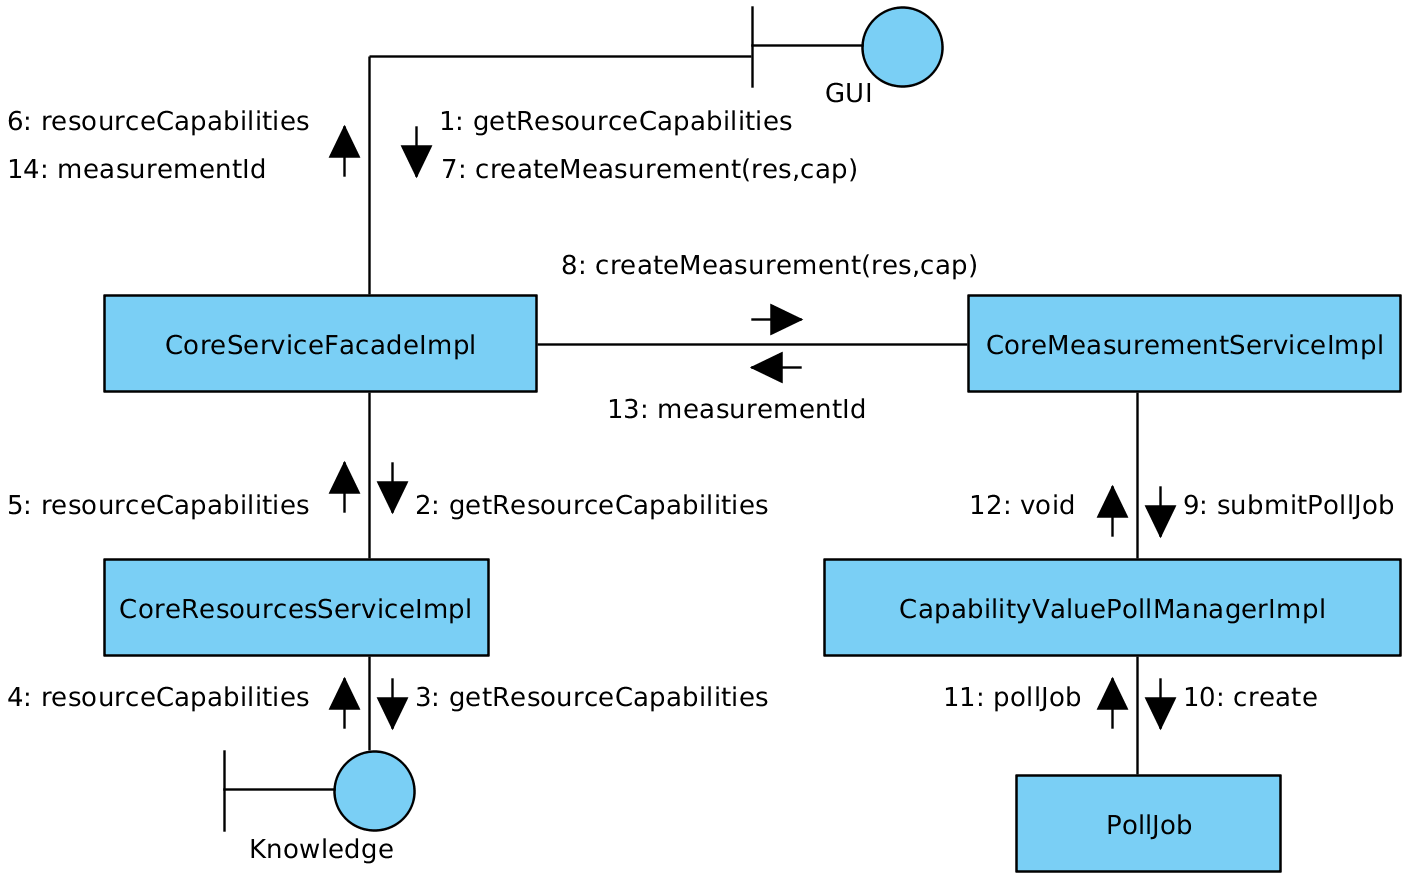
\includegraphics[width=0.8\textwidth]{comm_mh_add_measurement}
  \caption{Monitoring Hub Communication diagram - adding new measurement}
  \label{fig:comm_mh_add_measurement}
\end{figure}

Last data flow covered in this section describes gathering and publishing capability values. Action is initialized by
CapabilityValuePollManagerImpl. It's internal scheduler triggers previously created PollJob which contains measurement
definition (URI's of resource and capability). Using those identifiers, PollJob calls CoreMeasurementServiceImpl to
getCapabilityValue. Measurement service first lookups transport proxy using TransportProxiesManagerImpl and than, using
external TransportProxy, get capability value. In next step, gathered capability value is pushed to all listeners,
either directly (to listeners registered at CoreMeasurementServiceImpl) or using CoreRemoteServiceImpl to all remote
listeners. What should be noticed here is that CoreRemoteServiceImpl notifies remote listeners in asynchronous and
aggregated manner.

\begin{figure}[h]
  \centering
  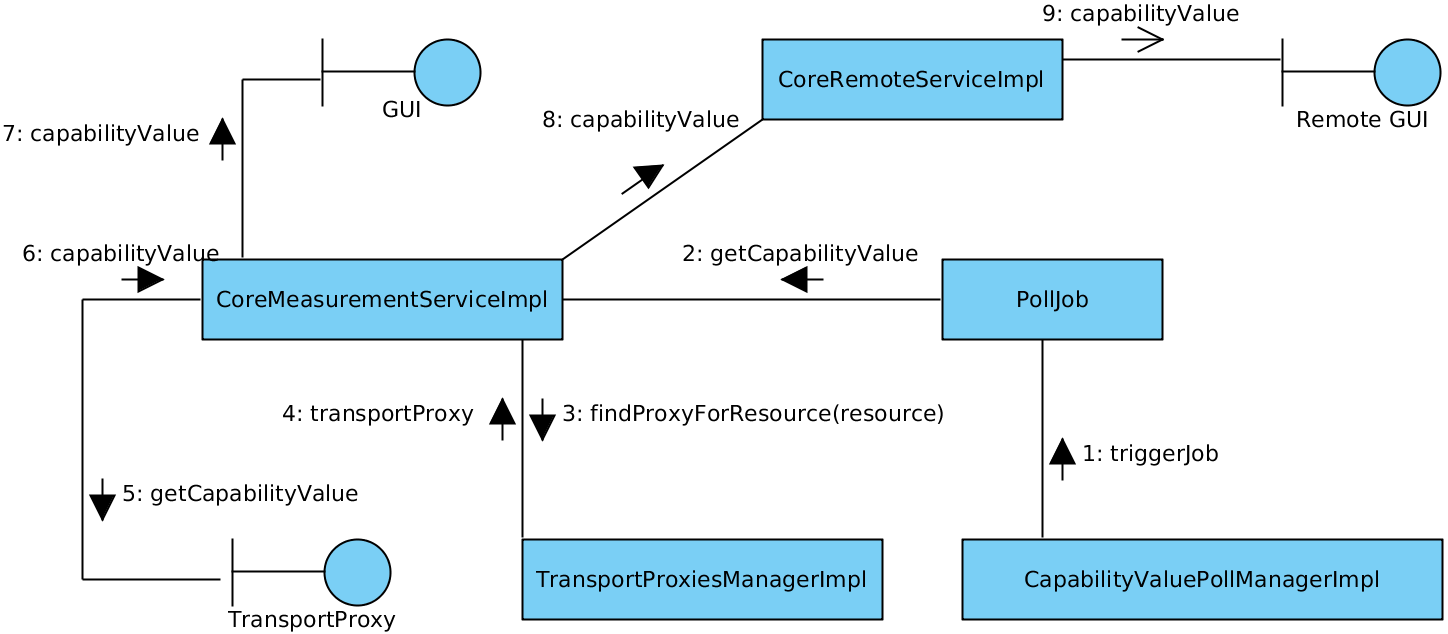
\includegraphics[width=1\textwidth]{comm_mh_new_cap_val}
  \caption{Monitoring Hub Communication diagram - new capability value notification}
  \label{fig:comm_new_cap_val}
\end{figure}

\pagebreak